\subsection{位似形}\label{subsec:czjh2-6-11}
\begin{enhancedline}

\begin{wrapfigure}[6]{r}{5cm}
    \centering
    \begin{tikzpicture}
    \tkzDefPoints{0/0/A, 4/0/B, 3.5/2.5/C, 1/3.6/D, 2/1.8/O}
    \foreach \n in {A,B,C,D} {
        \tkzDefPointOnLine[pos=2/3](O,\n)  \tkzGetPoint{\n'}
    }

    \tkzDrawPolygon(A,B,C,D)
    \tkzDrawPolygon(A',B',C',D')
    \tkzDrawSegments(O,A  O,B  O,C  O,D)
    \tkzLabelPoints[below](A,B)
    \tkzLabelPoints[right](C)
    \tkzLabelPoints[above](D)
    \tkzLabelPoints[below=.3em](O)
    \tkzLabelPoints[below](A')
    \tkzLabelPoints[below,xshift=-.3em](B')
    \tkzLabelPoints[below left](D')
    \tkzLabelPoints[below,xshift=-.5em](C')
\end{tikzpicture}


    \caption{}\label{fig:czjh2-6-39}
\end{wrapfigure}

现在,我们来研究相似形的一种特殊情形。

如图 \ref{fig:czjh2-6-39}, $O$ 是四边形 $ABCD$ 内的任一点, $A'$、$B'$、$C'$、$D'$ 分别是 $OA$、$OB$、$OC$、$OD$ 上的点。

$\dfrac{OA'}{OA} = \dfrac{OB'}{OB} = \dfrac{OC'}{OC} = \dfrac{OD'}{OD} = \exdfrac{2}{3}$。

可以证明四边形 $A'B'C'D' \xiangsi$ 四边形 $ABCD$, 并且相似比为 $\exdfrac{2}{3}$。

$\dfrac{OA'}{OA} = \dfrac{OB'}{OB} = \dfrac{OC'}{OC}$

\qquad $\tuichu \left\{\begin{aligned}
    A'B' \pingxing AB \tuichu \left\{\begin{aligned}
            \dfrac{A'B'}{AB} = \dfrac{OB'}{OB} = \exdfrac{2}{3} \\
            \angle OB'A' = \angle OBA
        \end{aligned}\right. \\
    B'C' \pingxing BC \tuichu \left\{\begin{aligned}
        \dfrac{B'C'}{BC} = \dfrac{OB'}{OB} = \exdfrac{2}{3} \\
        \angle OB'C' = \angle OBC
    \end{aligned}\right.
\end{aligned}\right\}$

\qquad $\tuichu \left\{\begin{aligned}
    \dfrac{A'B'}{AB} = \dfrac{B'C'}{BC} = \exdfrac{2}{3} \douhao \\
    \angle A'B'C' = \angle ABC \juhao
\end{aligned}\right.$

同理可得 $\dfrac{A'B'}{AB} = \dfrac{B'C'}{BC} = \dfrac{C'D'}{CD} = \dfrac{D'A'}{DA} = \exdfrac{2}{3}$,
$\angle B'C'D' = \angle BCD$, $\angle C'D'A' = \angle CDA$, $\angle D'A'B' = \angle DAB$。

$\therefore$ \quad $\text{四边形} \; A'B'C'D' \xiangsi \text{四边形} \; ABCD$, 相似比为 $\exdfrac{2}{3}$。

由此看出,在四边形 $ABCD$ 和四边形 $A'B'C'D'$ 中,如果有:
(1)对应顶点 $A'$ 和 $A$, $B'$ 和 $B$, $C'$ 和 $C$, $D'$ 和 $D$ 的连线都经过同一点 $O$;
(2)$\dfrac{OA'}{OA} = \dfrac{OB'}{OB} = \dfrac{OC'}{OC} = \dfrac{OD'}{OD} = \exdfrac{2}{3}$,
那么四边形 $A'B'C'D'$ 和四边形 $ABCD$ 相似,相似比等于 $\exdfrac{2}{3}$,
这样的两个四边形有特殊的位置关系。

如果一个图形上的点 $A'$、$B'$、$\cdots$、$P'$ 和另一个图形上的点 $A$、$B$、$\cdots$、$P$ 分别对应,并且

(1)直线 $A'A$、$B'B$、$\cdots$、$P'P$ 都经过同一点 $O$;

(2)$\dfrac{OA'}{OA} = \dfrac{OB'}{OB} = \cdots = \dfrac{OP'}{OP} = k$,\\
那么这两个图形叫做\zhongdian{位似图形},点 $O$ 叫做\zhongdian{位似中心}。

位似图形不仅形状相同,而且有特殊的位置关系。

对于两个多边形来说,只要它们的对应顶点 $A'$、$B'$、$\cdots$、$P'$ 和 $A$、$B$、$\cdots$、$P$ 有
上面的 (1)、(2) 两个关系,这两个多边形就是位似多边形。
如图 \ref{fig:czjh2-6-39} 中的四边形 $A'B'C'D'$ 和四边形 $ABCD$ 是位似四边形。

用类似的方法,可以证明(由同学自己证明):

\begin{xingzhi}
    两个位似多边形一定相似,它们的相似比等于对应顶点与位似中心的距离的比,它们的各对对应边分别平行。
\end{xingzhi}

两个位似图形的各对对应点可以全部都在位似中心的同旁,这时这两个位似图形叫做相互\zhongdian{外位似},位似中心叫做\zhongdian{外位似中心};
也可以全部都在位似中心的两旁,这时这两个位似图形叫做相互\zhongdian{内位似},位似中心叫做\zhongdian{内位似中心}。
例如,图 \ref{fig:czjh2-6-40} 中,五边形 $A'B'C'D'E'$ 和五边形 $ABCDE$ 相互外位似,点 $O$ 为外位似中心。
图 \ref{fig:czjh2-6-41} 中,五边形 $A'B'C'D'E'$ 和五边形 $ABCDE$ 相互内位似,点 $O$ 为内位似中心。

\begin{figure}[htbp]
    \centering
    \begin{minipage}[b]{7cm}
        \centering
        \begin{tikzpicture}
    \tkzDefPoints{0/0/A, 3/0/B, 2.7/1.4/C, 1.5/2/D, 0.8/2.1/E, -1.5/1/O}
    \foreach \n in {A,B,C,D,E} {
        \tkzDefPointOnLine[pos=.6](O,\n)  \tkzGetPoint{\n'}
    }

    \tkzDrawPolygon(A,B,C,D,E)
    \tkzDrawPolygon(A',B',C',D',E')
    \tkzDrawSegments[dashed](O,A  O,B  O,C  O,D  O,E)
    \tkzLabelPoints[below](A,B)
    \tkzLabelPoints[right](C)
    \tkzLabelPoints[above](D,E)
    \tkzLabelPoints[left](O)
    \tkzLabelPoints[below left](A')
    \tkzLabelPoints[below,xshift=-.3em,yshift=.2em](B')
    \tkzLabelPoints[below right](C')
    \tkzLabelPoints[above,xshift=.3em, yshift=-.2em](D')
    \tkzLabelPoints[above](E')
\end{tikzpicture}


        \caption{}\label{fig:czjh2-6-40}
    \end{minipage}
    \qquad
    \begin{minipage}[b]{7cm}
        \centering
        \begin{tikzpicture}
    \tkzDefPoints{0/0/A, 3/0/B, 2.7/1.4/C, 1.5/2/D, 0.8/2.1/E, -0.5/1/O}
    \foreach \n in {A,B,C,D,E} {
        \tkzDefPointOnLine[pos=1.5](\n,O)  \tkzGetPoint{\n'}
    }

    \tkzDrawPolygon(A,B,C,D,E)
    \tkzDrawPolygon(A',B',C',D',E')
    \tkzDrawSegments[dashed](A,A'  B,B'  C,C'  D,D'  E,E')
    \tkzLabelPoints[below](A,B)
    \tkzLabelPoints[right](C)
    \tkzLabelPoints[above](D,E)
    \tkzLabelPoints[above=.2em, xshift=.2em](O)
    \tkzLabelPoints[above](A')
    \tkzLabelPoints[left](B')
    \tkzLabelPoints[left](C')
    \tkzLabelPoints[below left](D')
    \tkzLabelPoints[below](E')
\end{tikzpicture}


        \caption{}\label{fig:czjh2-6-41}
    \end{minipage}
\end{figure}

\liti[0] 已知:锐角三角形 $ABC$(图 \ref{fig:czjh2-6-42})。

求作:矩形 $DEFG$, 使 $DE$ 在边 $BC$ 上,点 $G$ 和 $F$ 分别在边 $AB$ 和 $AC$ 上,且 $DE:GD = 2:1$。

\zuofa  1. 在 $AB$ 上任取一点 $G_1$, 作  $G_1D_1 \perp BC$,垂足为 $D_1$。

2. 在 $D_1C$ (或其延长线)上取一点 $E_1$,使 $D_1E_1 = 2 G_1D_1$。

3. 以 $G_1D_1$、$D_1E_1$ 为邻边作矩形 $D_1E_1F_1G_1$。

4. 作射线 $BF_1$, 交 $AC$ 于点 $F$。

5. 作 $FE \pingxing F_1E_1$, 交 $BC$ 于点 $E$;
   作 $FG \pingxing F_1G_1$, 交 $AB$ 于点 $G$;
   作 $GD \pingxing G_1D_1$, 交 $BC$ 于点 $D$。

四边形 $DEFG$ 就是所求的矩形。

\zhengming 由作法知, $DE$ 在 $BC$上, 点 $G$、$F$ 分别在 $AB$、$AC$ 上。

又 $DD_1$、$EE_1$、$FF_1$、$GG_1$ 相交于点 $B$,且
$$ \dfrac{BE}{BE_1} = \dfrac{BF}{BF_1} = \dfrac{BG}{BG_1} = \dfrac{BD}{BD_1} \douhao $$

$\therefore$ \quad 四边形 $DEFG$ 和四边形 $D_1E_1F_1G_1$ 位似。

$\therefore$ \quad 四边形 $D_1E_1F_1G_1$ 是矩形,且
$$ D_1E_1:G_1D_1 = 2:1 \douhao $$

$\therefore$ \quad 四边形 $DEFG$ 是矩形,且 $DE:GD = 2:1$。

\begin{figure}[htbp]
    \centering
    \begin{minipage}[b]{7cm}
        \centering
        \begin{tikzpicture}
    \tkzDefPoints{0/0/B, 4/0/C, 2.5/2.5/A}
    \tkzDrawPolygon(A,B,C)
    \tkzLabelPoints[above](A)
    \tkzLabelPoints[left](B)
    \tkzLabelPoints[right](C)

    % 1
    \tkzDefPointOnLine[pos=0.7](A,B)  \tkzGetPoint{G_1}
    \tkzDefLine[altitude](B,G_1,C)  \tkzGetPoint{D_1}
    \tkzDrawSegment(G_1,D_1)
    \tkzLabelPoints[left](G_1)
    \tkzLabelPoints[below,xshift=-.3em](D_1)

    % 2
    \tkzDefPointBy[rotation=center D_1 angle -90](G_1)  \tkzGetPoint{x}
    \tkzDefPointOnLine[pos=2](D_1,x)  \tkzGetPoint{E_1}
    \tkzLabelPoints[below](E_1)

    % 3
    \tkzDefPointBy[translation=from D_1 to E_1](G_1)  \tkzGetPoint{F_1}
    \tkzDrawPolygon(D_1,E_1,F_1,G_1)
    \tkzLabelPoints[below right](F_1)

    % 4
    \tkzInterLL(B,F_1)(A,C)  \tkzGetPoint{F}
    \tkzDrawSegment[dashed](B,F)
    \tkzLabelPoints[right](F)

    % 5
    \tkzDefLine[parallel=through F](F_1,E_1)  \tkzGetPoint{e}
    \tkzInterLL(F,e)(B,C)  \tkzGetPoint{E}
    \tkzDefLine[parallel=through F](F_1,G_1)  \tkzGetPoint{g}
    \tkzInterLL(F,g)(A,B)  \tkzGetPoint{G}
    \tkzDefLine[parallel=through G](G_1,D_1)  \tkzGetPoint{d}
    \tkzInterLL(G,d)(B,C)  \tkzGetPoint{D}
    \tkzDrawPolygon(D,E,F,G)
    \tkzLabelPoints[below](D,E)
    \tkzLabelPoints[left](G)
\end{tikzpicture}


        \caption{}\label{fig:czjh2-6-42}
    \end{minipage}
    \qquad
    \begin{minipage}[b]{7cm}
        \centering
        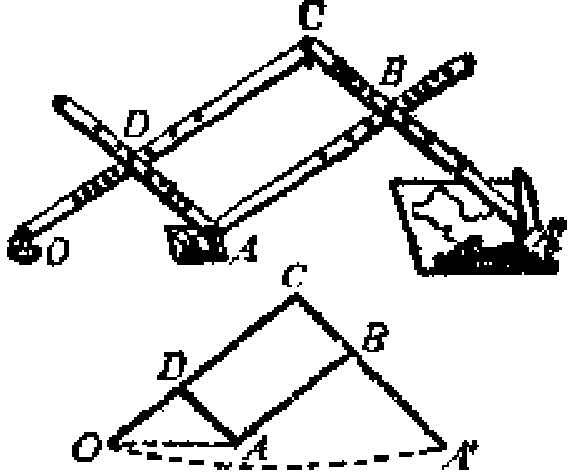
\includegraphics[width=5cm]{../pic/czjh2-ch6-43.png}
        \caption{}\label{fig:czjh2-6-43}
    \end{minipage}
\end{figure}


实际画图使用的一种工具——放缩尺,就是根据已知图形作出它的位似图形的道理制成的。
应用它可以按指定的比把各种图形进行放大或缩小。如图 \ref{fig:czjh2-6-43},
把钻有若干小孔的四条直尺用螺栓分别在点 $A$、$B$、$C$、$D$ 连接起来,
使直尺可以绕着这些点转动,并使
$$ OD = DA = CB \douhao DC = AB = BA' \juhao $$

根据以上构造可知:不论直尺如何转动,四边形 $ABCD$ 总是平行四边形,
而 $\triangle ODA$ 和 $\triangle OCA'$ 都是等腰三角形,并且
\begin{gather*}
    \angle ODA = \angle OCA' \douhao \\
    \angle ODA = \exdfrac{1}{2} (180^\circ - \angle ODA) = \exdfrac{1}{2} (180^\circ - \angle OCA') = \angle COA' \juhao
\end{gather*}

从而得点 $O$、$A$、$A'$ 在同一直线上。
$$ \dfrac{OA'}{OA} = \dfrac{OC}{OD} = k \text{, 或} \quad \dfrac{OA}{OA'} = \dfrac{OD}{OC} = \exdfrac{1}{k} \juhao $$
于是,当点 $O$ 的位置固定时,不论各尺如何转动,
点 $A'$ 和 $A$ 都是以点 $O$ 为外位似中心,以 $k$ 为相似比的外位似图形的对应点,
点 $A$ 和 $A'$ 都是以   $O$ 为外位似中心,以 $\exdfrac{1}{k}$ 为相似比的外位似图形的对应点。

当我们放大某一给定图形时,将这个图形固定在点 $A$ 处的下方,在尺上的点 $A$ 处装上尖针;
将空白的图纸固定在点 $A'$ 处的下方,在尺上的点 $A'$ 处装上画图笔。
当尺上的尖针 $A$ 沿所给的图形移动时,尺上点 $A'$ 处的画图笔尖就可以在空白图纸上画出
把所给图形放大成原来的 $\dfrac{OC}{OD}$ 倍的图形。

交换上述的尖针与画笔的位置,也交换所给图形与空白图纸的位置,
就可以画出把所给图形缩小成原来的 $\dfrac{OD}{OC}$ 的图形。

改变螺栓所在的小孔 $B$ 和 $D$,可以调整放大或缩小的比。


\begin{lianxi}

\xiaoti{作一个四边形 $A'B'C'D'$ 和已知四边形 $ABCD$ 外位似,相似比 $k = \exdfrac{3}{4}$,
    外位似中心取在(1)$ABCD$ 的外部; (2) $ABCD$ 的一条边上; (3)$ABCD$ 的一个顶点。
}

\xiaoti{作一个四边形 $A'B'C'D'$ 和已知四边形 $ABCD$ 内位似,相似比 $k = \exdfrac{3}{4}$,
    內位似中心取在 $ABCD$ 的 (1)外部; (2)内部。
}

\end{lianxi}
\end{enhancedline}

